\documentclass[11pt,a4paper]{article}

\usepackage[margin=2.5cm]{geometry}
\usepackage{amsmath,amssymb,amsthm}
\usepackage{booktabs}
\usepackage{graphicx}

\newtheorem{proposition}{Proposition}[section]
\newtheorem{theorem}[proposition]{Theorem}

\newcommand{\R}{\mathbb{R}}
\newcommand{\Z}{\mathbb{Z}}
\newcommand{\Q}{\mathbb{Q}}

\title{\textbf{The Unbalanced Dual Matching Coefficients:\\
$\boldsymbol{\Gamma(\tfrac14+ix)\,\Gamma(\tfrac34-ix)}$}}
\author{Robin Langer and Claude Code}
\date{August 2026}

\begin{document}
\maketitle

%% ===================================================================
\section{The Kernel and Its Shift}
%% ===================================================================

Consider the \emph{bilinear} pairing $\langle f, g\rangle = \int_\R f\,g\,dx$
(no conjugation) and the kernel
\[
  W(x) = \Gamma(\tfrac14 + ix)\,\Gamma(\tfrac34 - ix).
\]
By the reflection formula $\Gamma(s)\Gamma(1-s) = \pi/\sin\pi s$
with $s = \tfrac14 + ix$,
\begin{equation}\label{eq:reflection}
  W(x) = \frac{\pi}{\sin\pi(\tfrac14 + ix)},
\end{equation}
which is \emph{complex-valued}, with $W(-x) = \overline{W(x)}$.
In particular $W$ is not a positive weight and no Hermitian
orthogonal polynomials exist---this is genuine dual-basis territory.

\medskip
\noindent\textbf{The shift.}
The imaginary translation $y = x + \tfrac{i}{4}$ maps the kernel to
\[
  W(y - \tfrac{i}{4})
  = \Gamma(\tfrac12 + iy)\,\Gamma(\tfrac12 - iy)
  = \bigl|\Gamma(\tfrac12 + iy)\bigr|^2,
\]
the standard weight for Meixner--Pollaczek polynomials with
$\lambda = \tfrac12$, $\phi = \tfrac\pi2$.  This reduces the
bilinear problem to a shifted copy of a classical self-dual case.

Specifically, let $P_n$ denote the standard MP($\tfrac12$, $\tfrac\pi2$)
polynomials, satisfying
\[
  (n+1)\,P_{n+1}(y) = 2y\,P_n(y) - n\,P_{n-1}(y),
  \qquad P_0 = 1, \quad P_1 = 2y,
\]
with norms $h_n^{\mathrm{std}} = \int_\R P_m P_k\,|\Gamma(\tfrac12+iy)|^2\,dy
= \pi\,\delta_{mk}$ (all norms equal~$\pi$).
Then $Q_n(x) := P_n(x + \tfrac{i}{4})$ are the monic bilinear
orthogonal polynomials for~$W$:
\[
  \int_\R Q_m(x)\,Q_k(x)\,W(x)\,dx = \pi\,\delta_{mk}.
\]
The monic versions $q_n = (n!/2^n)\,Q_n$ satisfy the three-term
recurrence
\begin{equation}\label{eq:recurrence}
  q_{n+1} = \bigl(x + \tfrac{i}{4}\bigr)\,q_n
  - \bigl(\tfrac{n}{2}\bigr)^2 q_{n-1},
  \qquad
  h_n^{\mathrm{monic}}
  = \pi\,\frac{(n!)^2}{4^n}.
\end{equation}
(Verified numerically to $50$ digits for $n \le 11$.)

%% ===================================================================
\section{Moments}
%% ===================================================================

The two-Gamma integral formula gives the moment generating function.
With $a = \tfrac14$, $b = \tfrac34$,
\begin{equation}\label{eq:mgf}
  \int_\R W(x)\,e^{isx}\,dx
  = 2\pi\,\frac{e^{3s/4}}{1 + e^s}\,,
\end{equation}
so $\mu_0 = \pi$, and the moments $\mu_n = \int x^n W\,dx$ are
obtained by differentiating: $\mu_n = (-i)^n F^{(n)}(0)$ where
$F(s) = 2\pi e^{3s/4}/(1+e^s)$.  Even moments are real, odd moments
purely imaginary (from $W(-x) = \overline{W(x)}$), and the Hankel
determinants $\Delta_n = \det(\mu_{j+k})_{0 \le j,k < n}$ are all
real and positive (verified for $n \le 12$), confirming existence
of the bilinear orthogonal polynomials.

%% ===================================================================
\section{The Three-Gamma Matching Integral}
%% ===================================================================

Split $W = w_+\,w_-$ with $w_+ = \Gamma(\tfrac14+ix)$,
$w_- = \Gamma(\tfrac34-ix)$.  The normalised dual functions are
\[
  F_m = w_+\,\widehat{P}_m, \qquad G_m = w_-\,\widehat{P}_m,
\]
biorthonormal: $\int F_m\,G_k\,dx = \delta_{mk}$ (verified to
$50$~digits for $m,k \le 6$).  The matching coefficients
\[
  c_{mk} = \langle F_m, \widehat{P}_k\rangle_W
  = \frac{J_{mk}}{\pi}, \qquad
  J_{mk} = \int_\R P_m\bigl(x+\tfrac{i}{4}\bigr)\,
    P_k\bigl(x+\tfrac{i}{4}\bigr)\;
    \Gamma\bigl(\tfrac14+ix\bigr)^2\,
    \Gamma\bigl(\tfrac34-ix\bigr)\,dx,
\]
are computed by the three-Gamma integral (Proposition~1 of the
companion paper) with $a = b = \tfrac14$, $c = \tfrac34$:
\begin{equation}\label{eq:base}
  J_{00}
  = 2\pi\,\Gamma(1)^2\,U(1, 1, 1)
  = 2\pi\,e\,E_1(1)
  = 3.74696098492\ldots
\end{equation}
using $U(1,1,z) = e^z\,E_1(z)$ (Tricomi's function in terms
of the exponential integral).

%% ===================================================================
\section{The Master Generating Function}
%% ===================================================================

Substituting the polynomial generating function
$\sum P_n(y)\,w^n = (1-iw)^{-1/2+iy}(1+iw)^{-1/2-iy}$
with $y = x + \tfrac{i}{4}$ into the matching integral and
using the shifted three-Gamma formula~(equation~(2) of the
companion paper),
\begin{equation}\label{eq:gf}
  \boxed{
  \sum_{m,k \ge 0} J_{mk}\,w^m u^k
  = \frac{2\pi\,e^{\eta}\,E_1(\eta)}{(1-iw)(1-iu)}\,,
  \qquad
  \eta = \frac{(1+iw)(1+iu)}{(1-iw)(1-iu)}\,.
  }
\end{equation}
At $w = u = 0$, $\eta = 1$, recovering~\eqref{eq:base}.
Verified numerically to $15$ digits against all $78$ entries of
the $12 \times 12$ table.

\subsection*{Comparison with the self-dual case}

The companion paper's generating function for
$W_0 = |\Gamma(\tfrac14+ix)|^2$ (the self-dual MP($\tfrac14$) case) was
\[
  \frac{2\pi^{3/2}\,e^{\zeta/2}\,K_0(\zeta/2)}
       {\sqrt{(1-iw)(1-iu)}}\,,
  \qquad
  \zeta = \varphi(w)\,\varphi(u)\,,
\]
with $\varphi$ the Cayley transform and the modified Bessel function
$K_0$.  The structural differences are summarised:

\begin{center}
\small
\begin{tabular}{@{}lp{5.5cm}p{5.5cm}@{}}
\toprule
 & Self-dual ($\lambda = \tfrac14$) & Unbalanced ($\lambda = \tfrac12$ shifted) \\
\midrule
Special fn & $K_0(\zeta/2)$ & $E_1(\eta)$ \\
ODE order & $2$ (Bessel) & $1$ (first-order) \\
Generators & $2$: $A = \sqrt{2e}\,K_0(\tfrac12)$,
              $B = \sqrt{2e}\,K_1(\tfrac12)$
            & $1$: $A = e\,E_1(1)$ \\
Prefactor & $1/\sqrt{(1-iw)(1-iu)}$ & $1/\bigl((1-iw)(1-iu)\bigr)$ \\
Variable & $\zeta = \varphi(w)\varphi(u)$ &
  $\eta = \frac{(1+iw)(1+iu)}{(1-iw)(1-iu)}$ \\
\bottomrule
\end{tabular}
\end{center}

\subsection*{Single-generator structure}

The derivative algebra of $f(z) = e^z E_1(z)$ is first-order:
\[
  f'(z) = f(z) - \frac{1}{z},
\]
so $f^{(n)}(1) \in \Q\cdot A \oplus \Q$ for all $n$ by induction.
Since the Taylor coefficients of~\eqref{eq:gf} are polynomial
expressions in the derivatives of $f$ at $z = 1$, every matching
coefficient lies in $\Q\,A \oplus \Q$:
\begin{equation}\label{eq:integrality}
  \frac{J_{mk}}{2\pi}
  \in (\Q\,A \oplus \Q) \cdot i^{m+k},
  \qquad A = e\,E_1(1) = 0.59634736\ldots
\end{equation}
This contrasts with the self-dual case, where the Bessel ODE
is second-order and produces \emph{two} independent generators.
The structural reason: $E_1$ satisfies $z E_1' + E_1 = e^{-z}/z$,
a first-order inhomogeneous equation, while $K_0$ satisfies
$z^2 K_0'' + z K_0' - z^2 K_0 = 0$, a second-order equation whose
solution space is two-dimensional.

\subsection*{Parity}

Since $W(-x) = \overline{W(x)}$, substituting $x \mapsto -x$
gives $J_{mk} = (-1)^{m+k}\overline{J_{mk}}$: entries with
$m+k$ even are real, odd are purely imaginary.  The self-dual
case had the same checkerboard; the kernel's asymmetry does
not break~it.

%% ===================================================================
\section{The Coefficient Table}
%% ===================================================================

The table lists $J_{mk}/(2\pi)$ decomposed over the single
generator $A = e\,E_1(1)$.  A factor of~$i$ is suppressed for
$m+k$ odd.

\begin{table}[ht]
\centering
\small
\begin{tabular}{cl@{\qquad}cl}
\toprule
$(m,k)$ & $J_{mk}/(2\pi)$ & $(m,k)$ & $J_{mk}/(2\pi)$ \\
\midrule
$(0,0)$ & $A$                         & $(1,3)$ & $87A - 52$ \\
$(0,1)$ & $3A - 2$                    & $(1,4)$ & $\tfrac{547}{3}A - \tfrac{326}{3}$ \\
$(0,2)$ & $-7A + 4$                   & $(2,2)$ & $121A - 72$ \\
$(0,3)$ & $-\tfrac{43}{3}A + \tfrac{26}{3}$  & $(2,3)$ & $\tfrac{949}{3}A - \tfrac{566}{3}$ \\
$(0,4)$ & $27A - 16$                  & $(2,4)$ & $-\tfrac{2167}{3}A + \tfrac{1292}{3}$ \\
$(0,5)$ & $\tfrac{719}{15}A - \tfrac{86}{3}$ & $(3,3)$ & $-\tfrac{8101}{9}A + \tfrac{4832}{9}$ \\
$(1,1)$ & $-13A + 8$                  & $(3,4)$ & $-\tfrac{6617}{3}A + \tfrac{3946}{3}$ \\
$(1,2)$ & $-37A + 22$                 & $(4,4)$ & $\tfrac{51649}{9}A - \tfrac{30800}{9}$ \\
\bottomrule
\end{tabular}
\end{table}

All PSLQ identifications verified to $40+$ digits.  The matching
coefficients of $F_m$ are $c_{mk} = J_{mk}/\pi$; those of $G_m$
are the complex conjugates.

%% ===================================================================
\section{The Reverse Expansion}
%% ===================================================================

The reverse coefficients
$D_{mk} = \int \widehat{P}_m\,G_k\,dx$
involve a single Gamma factor.  The one-Gamma Fourier pair gives
\[
  \int_\R \Gamma(\tfrac34 - ix)\,e^{isx}\,dx
  = 2\pi\,e^{3s/4}\,e^{-e^s},
\]
and the generating function for the reverse table is
\begin{equation}\label{eq:gfrev}
  \sum_{m,k} \Bigl(\int P_m P_k\,\Gamma(\tfrac34-ix)\,dx\Bigr)
  w^m u^k
  = \frac{2\pi\,e^{-1/\eta}}{(1-iw)(1-iu)}\,,
\end{equation}
with $\eta$ as before.  At $w = u = 0$: $2\pi/e$.  The single
generator is now $e^{-1}$---the exponential integral has vanished,
leaving pure exponential arithmetic.  Every reverse coefficient
is a Gaussian rational times $2\pi/e$, provably so from the
Taylor expansion.

First entries of $R_{mk}/(2\pi/e)$, with $i$ suppressed for
$m+k$ odd:
\[
  \begin{pmatrix}
  1 & \frac12 & \frac12 & -\frac14 & \frac12 & -\frac{11}{4} \\[3pt]
    & \frac34 & \frac14 & \frac{13}{8} & -\frac{15}{4} & -\frac{49}{8} \\[3pt]
    &         & \frac94 & -\frac{25}{8} & \frac14 & -\frac{171}{8}
  \end{pmatrix}
\]

%% ===================================================================
\section{Zeros}
%% ===================================================================

\begin{figure}[ht]
\centering
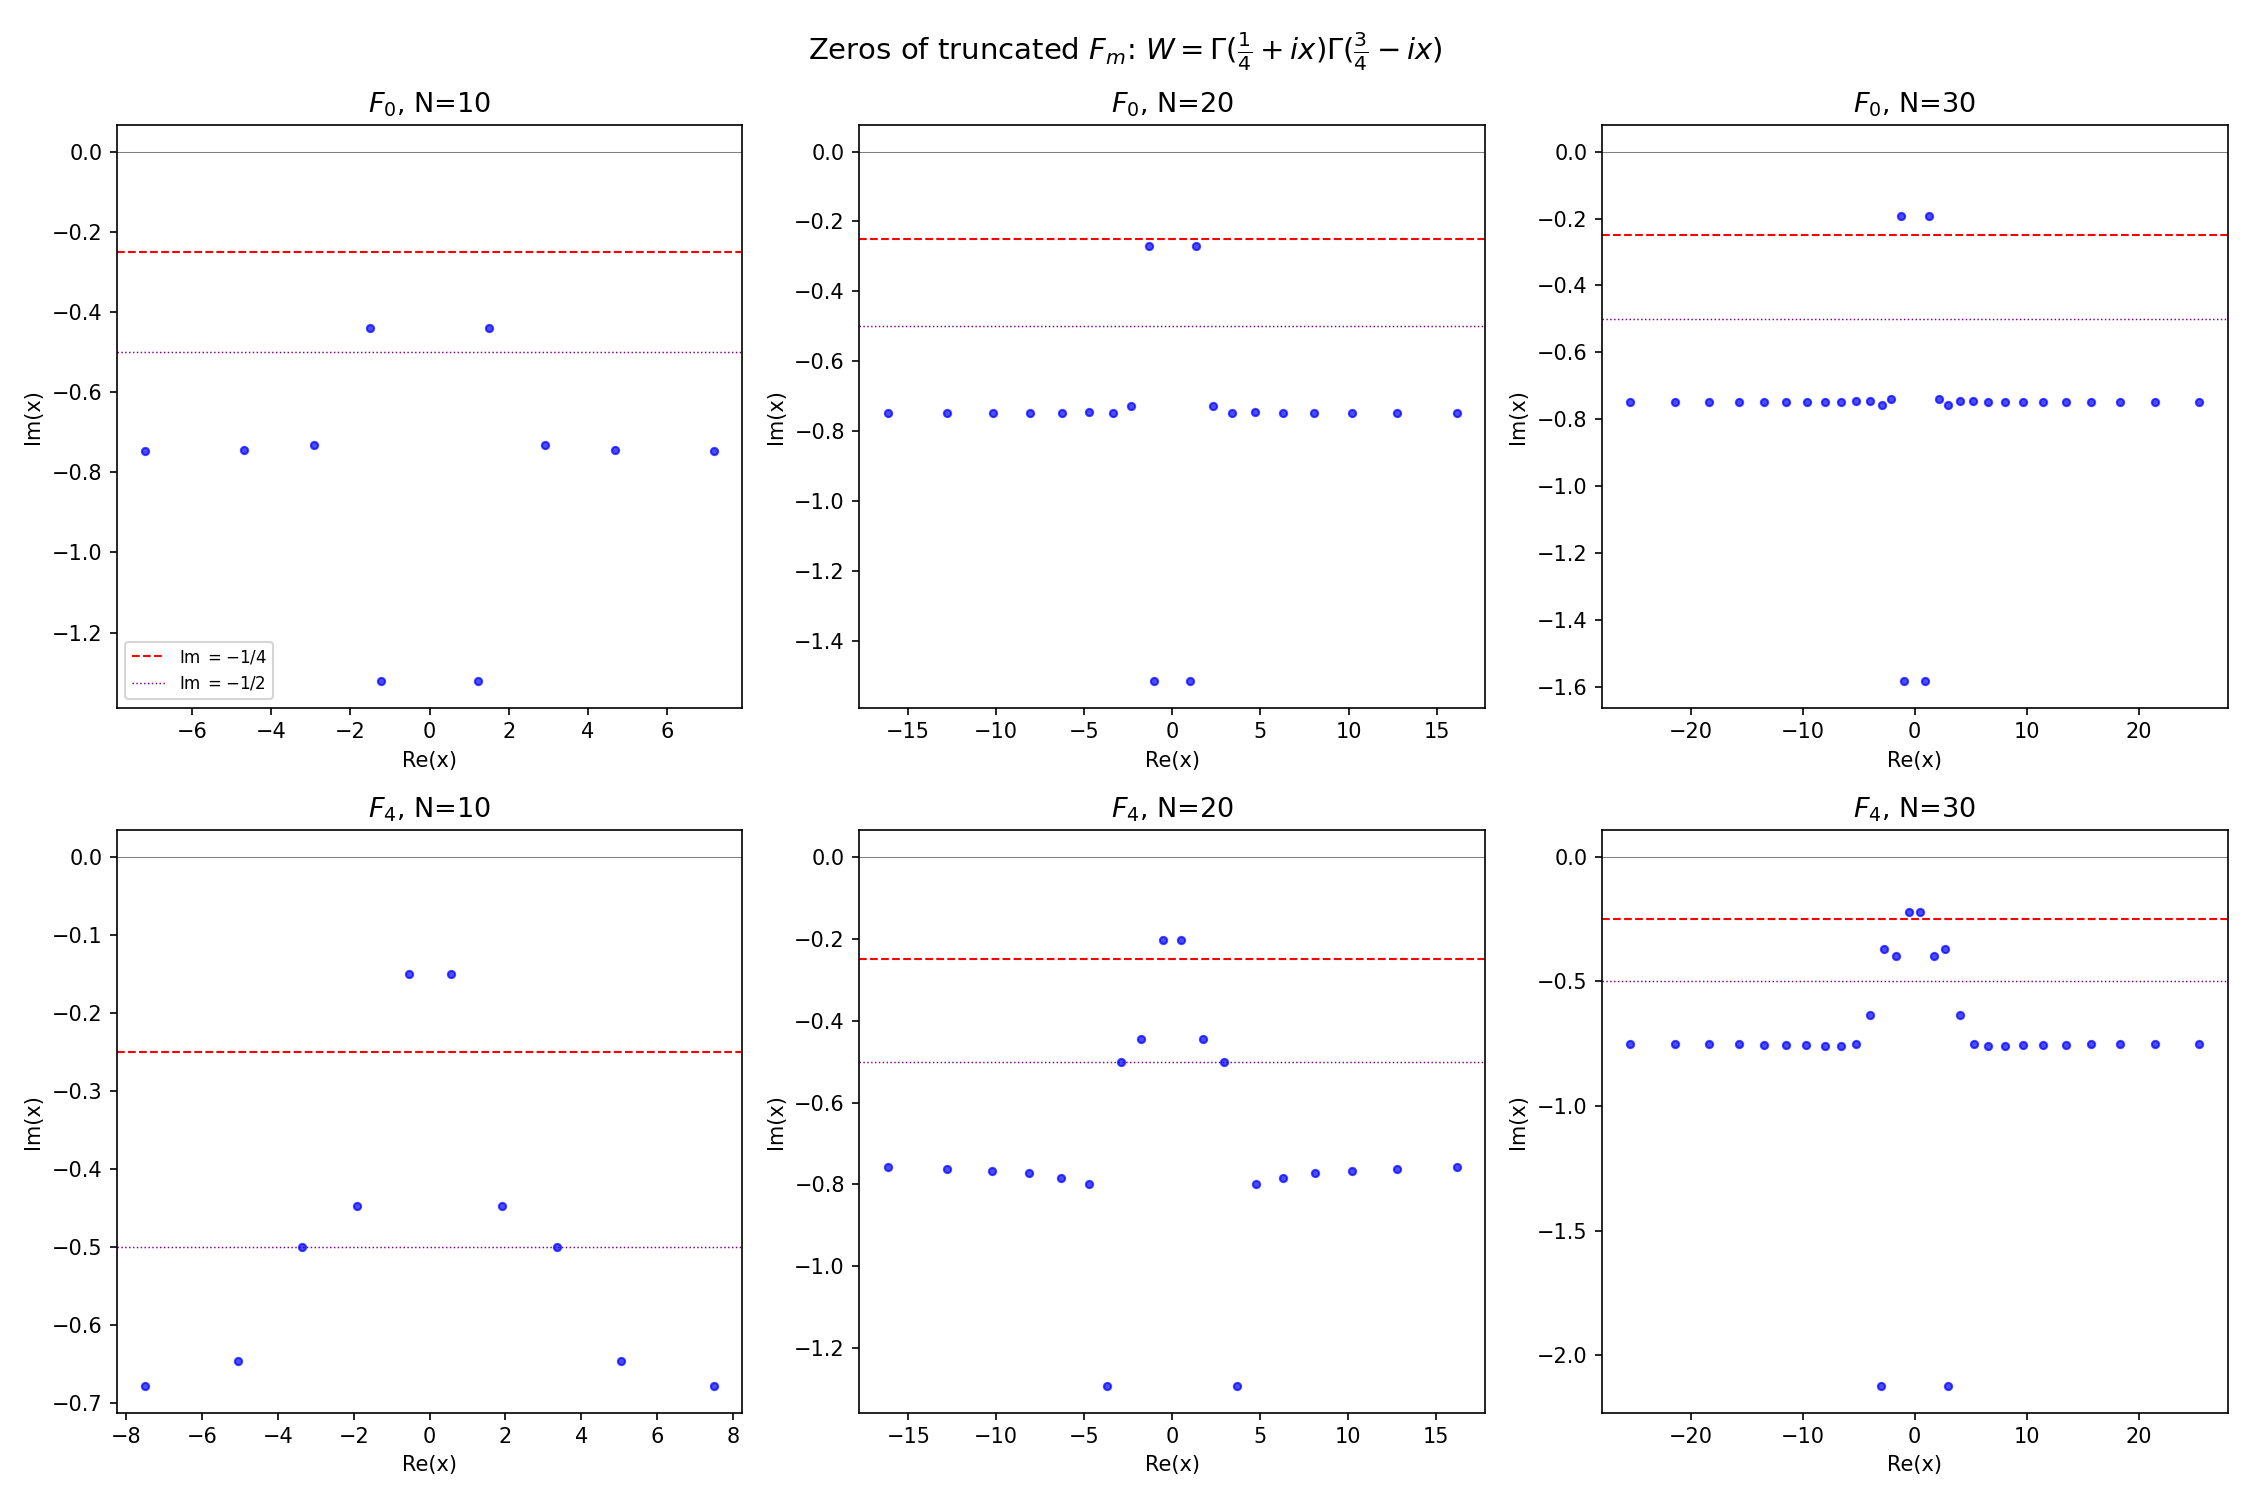
\includegraphics[width=0.95\textwidth]{unbalanced_zeros.png}
\caption{Zeros of the truncated dual functions
$\sum_{k \le N} c_{mk}\,\widehat{P}_k$ for $m = 0$ (top) and
$m = 4$ (bottom), at truncation orders $N = 10, 20, 30$.
The bulk of the spurious zeros lie in a band near
$\operatorname{Im} x \approx -0.7$, close to the nearest pole
line $\operatorname{Im} x = -\tfrac34$ of
$\Gamma(\tfrac34-ix)$.}
\label{fig:zeros}
\end{figure}

In the self-dual case $W_0 = |\Gamma(\tfrac14+ix)|^2$, the spurious
zeros of the polynomial approximation concentrated on the line
$\operatorname{Im} x = -\tfrac12$, midway between the pole ladders
at $\pm i(\tfrac14 + \Z_{\ge 0})$.  Here the pole ladders are
asymmetric:
\[
  w_+ = \Gamma(\tfrac14+ix): \quad
  \text{poles at } x = i(\tfrac14 + n), \quad n \ge 0,
\]
\[
  w_- = \Gamma(\tfrac34-ix): \quad
  \text{poles at } x = -i(\tfrac34 + n), \quad n \ge 0.
\]
The nearest pole to the real axis from \emph{below} is at
$\operatorname{Im} x = -\tfrac34$, and Figure~\ref{fig:zeros}
shows the bulk zeros cluster near this line rather than at the
midpoint $-\tfrac14$.  The zero-band is pulled towards the
nearer $w_-$~pole ladder, reflecting the asymmetry of the kernel.

%% ===================================================================
\section{Discussion}
%% ===================================================================

The unbalanced kernel $\Gamma(\tfrac14+ix)\,\Gamma(\tfrac34-ix)$
illustrates three phenomena:

\begin{enumerate}
\item \textbf{Reduction by shift.}  Every kernel
  $\Gamma(\lambda+ix)\,\Gamma(1-\lambda-ix)$ for
  $0 < \lambda < 1$ reduces via $y = x + i(\tfrac12-\lambda)$
  to the self-dual weight $|\Gamma(\tfrac12+iy)|^2$, i.e.\ the
  MP($\tfrac12$) case.  The ``unbalanced'' appearance is an
  artifact of the real-line presentation.

\item \textbf{First-order vs.\ second-order.}  The exponential
  integral $E_1$ replaces the Bessel function $K_0$ of the
  self-dual ($\lambda = \tfrac14$) case.  The derivative
  algebra collapses from a two-state automaton ($K_0 \leftrightarrow K_1$)
  to a one-state system ($A \mapsto A - 1$), halving the number
  of generators.  The structural reason is the ODE order:
  $K_\nu$ satisfies a second-order Bessel equation, while
  $E_1$ satisfies a first-order equation.

\item \textbf{Zeros geometry.}  The spurious zero band shifts
  from $\operatorname{Im} x = -\tfrac12$ (self-dual) to
  $\operatorname{Im} x \approx -\tfrac34$ (unbalanced),
  tracking the nearer pole ladder of the split.
\end{enumerate}

The broader family $\Gamma(\lambda+ix)\,\Gamma(\mu-ix)$ with
$\lambda + \mu = 1$ (reflection constraint) always reduces to
MP($\tfrac12$) by translation, but when $\lambda + \mu \ne 1$
the situation is genuinely different---the three-Gamma integral
involves $U(\alpha, \beta, 1)$ with $\alpha \ne \tfrac12$ and
the Bessel/exponential-integral correspondence breaks.  This
will be addressed in a sequel.

\end{document}
